\documentclass[12pt,UTF8,a4]{article}
\usepackage{amsmath, amssymb}
\usepackage{indentfirst}
\usepackage{multirow}
\usepackage{titlesec}
\usepackage{graphicx}
\usepackage{longtable}
\usepackage{framed}
\usepackage[noend]{algorithmic}
\usepackage{algorithm}
\usepackage{sectsty}
\usepackage{setspace}
\usepackage[footnotesize]{caption}
\usepackage{enumitem}
\usepackage[text={18cm,24cm}]{geometry}
\usepackage[hyperfigures,bookmarksnumbered,bookmarksopen,bookmarks,colorlinks,citecolor=blue,linkcolor=blue]{hyperref}
\usepackage{natbib}
\usepackage{mathpartir}

\setlength{\bibsep}{0.0pt}
\algsetup{indent=2em}
\setlength{\parindent}{2em} \setlength{\parskip}{3pt plus1pt minus1pt}

\DeclareGraphicsExtensions{.pdf,.png,.jpg}

\newcommand{\code}[1]{\texttt{#1}}
\newcommand{\type}[1]{\texttt{#1}}


\sectionfont{\large}
\subsectionfont{\normalsize}
\paragraphfont{\small}

\singlespacing
\title{CSCE 604 Final Project Report \\ Design and Implementation of a 2D Programming Language}
\author{Robert Schumacher, Plamen Ivanov and Peihong Guo}
\date{\today}

\begin{document}
\maketitle
\singlespacing

\tableofcontents

\section{Introduction}
We designed and implemented a two dimensional programming language
featuring an interactive web-based graphical programming environment.
This language features recursion, control flow branching,
parameterized types and type inference.

%% \section{Design Decisions}
%% \subsection{Language Specification}
%% \subsubsection{Visual Grammar}
%% The main element of the visual grammar are called "components". Each
%% component is described by a type signature. For example, an \code{if}
%% component may be given the following type signature:

%% \[ \forall \alpha.\ \type{bool} \rightarrow \alpha \rightarrow \alpha \rightarrow \alpha \]

%% Components are composed of an input, output, a name (if applicable)
%% and a body.  An input (or output) can be a tuple of any size composed
%% of valid data types. An output from one component will serve as a feed
%% for the input of another. Input and Outputs of different type will not
%% be compatible allowing for a way for components to be strung together
%% correctly.  The body of a component can be composed of any number of
%% other components, as long as they are connected correctly and provide
%% an output for the containing component. Using such components, the
%% programmer will be able to visually construct a program. The resulting
%% structure of connected components will have the form of a graph. The
%% graph will represent the structure of the program much better than
%% sequentially written code.  Places for parallelizing will be apparent
%% from simply viewing the graph. Components will form nodes in the graph
%% and connections between output and input will form edges. The graph
%% will also have a recursive structure as individual nodes can be
%% composed of large graphs themselves.

%% This visual language will need to be pure. This is necessary since,
%% there are no guarantees for the sequence of execution of some possible
%% programs. If side effects are allowed, it will be very difficult to
%% keep track of them or debug the resulting programs.

%% The following figure is an example of how we envision the graphical
%% language will look like:

%% This figure demonstrates the input/output matching and the definition
%% of a function SUM-TUPLE, which takes a tuple of two Integers and
%% returns their sum.

%% Translation:

%% The visual language above will have to be translated to a regular
%% language. The main step for doing this will be to serialize the graph
%% formed by the visual language. We can do that by using a topological
%% sorting of the nodes in the graph. It has to be noted that topological
%% sorting can result in many valid sorts. Additional rules may be needed
%% to ensure an efficient translation.


%% Regular Grammar:

%% The visual language will be translated into a regular language. We can use a basic language which  supports a few data types, such as Integers, Boolean, String and Tuples. Some of the details of the language to translate into are still in the process of development.

%% ====================================

\section{The Language}
\subsection{Programs}
A program in the 2D programming language is a collection of
functions. A function is the basic building block, which is a
collection of nodes: predefined functions, special nodes and user
defined functions. Special nodes include \code{input}, \code{output},
\code{if}, \code{constant} and \code{arithmetic}.
\begin{table}[!ht]
\center
\begin{tabular}{l|l}
\hline
Name & Usage \\
\hline
\code{input} & defines a parameter for a function \\
\code{output} & the output of a function\\
\code{if} & branching \\
\code{constant} & constant value (\type{string}, \type{number}, or \type{bool}) \\
\code{arithmetic} & an arithmetic calculation \\
\code{recursion} & recursion into the current function unit \\
\hline
\end{tabular}
\caption{Special nodes.}\label{tab:sitems}
\end{table}

Predefined functions include \code{print}, \code{pair}, \code{fst},
\code{snd}, \code{StringOfNumber}, \code{StringOfBool}, \code{Single},
\code{Nil}, \code{Head}, \code{Tail}, \code{Length}, \code{Append} and
\code{Concat}.
\begin{table}[!ht]
\center
\begin{tabular}{l|l}
\hline
Name & Usage \\
\hline
\code{print} & print the content passed to its input node\\
\code{pair} & make a pair out of its two inputs\\
\code{fst} & break a pair and take its first item \\
\code{snd} & break a pair and take its second item \\
\code{StringOfNumber} & convert a number into a string\\
\code{StringOfBool} & convert a boolean value into a string \\
\code{Single} & return a singleton list containing the argument \\
\code{Nil} & return an empty list \\
\code{Head} & return the first element in a list\\
\code{Tail} & return the list without its firts element\\
\code{Length} & returns the length of a list\\
\code{Append} & add an element to a list \\
\code{Concat} & concatenate two lists \\
\hline
\end{tabular}
\caption{Predefined items.}\label{tab:pitems}
\end{table}

The system maintains a global list of function definitions, including
predefined ones and user-defined ones. Each definition in the list has
a unique id, which is used as an identifier when they are
referenced. These definitions also contain links to the executable
code used during evaluation. For special definitions, new instances of
them will be created whenever they are added to a user-defined
definition. Predefined definitions are treated in the same way as
special definitions to simplify the implementation, though they behave
exactly the same as user-defined definitions.

\subsection{Functions}
Each function definition consists of inputs, an output, and zero or
more body nodes. The body of a definition may include other
definitions, such as predefined functions or user-defined functions.

The input of a node can be empty, which corresponds to a node that
does not require an input. Definitions of this type are \code{input},
\code{constant}, or functions which calculate constant values.

The body of a definition is a set of nodes referring to
definitions. The member nodes of a definition are connected by a set
of edges indicating the input-output dependencies between nodes, as is
shown in Figure~\ref{fig:defbody}.

\begin{figure}[!ht]
\center
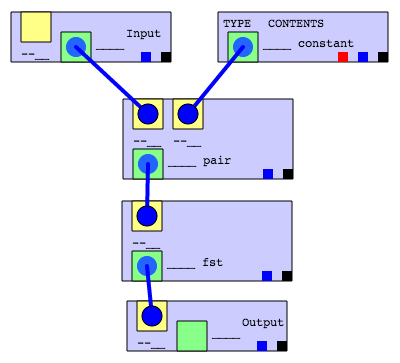
\includegraphics[width=0.5\textwidth]{./images/defbody}
\caption{The body of a definition for \code{identity} function.}\label{fig:defbody}
\end{figure}

Note the input and output nodes in Figure~\ref{fig:defbody} determines
the input this definition is taking and the output of this
definitions. A single input node indicates this definition, which is
essentially an identity function, takes only one input. If multiple
input nodes are included in the definition body, the function being
defined takes a number of inputs.

A node in the body of a definition can be a reference to a
user-defined function, as is shown in Figure~\ref{fig:ref}. Here the
\code{identity} node is a reference to the function defined in
Figure~\ref{fig:defbody}.
\begin{figure}[!ht]
\center
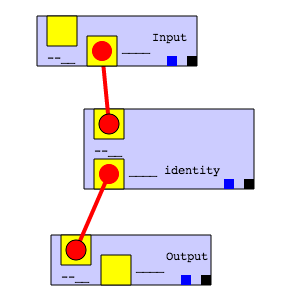
\includegraphics[width=0.35\textwidth]{./images/ref} \\
\caption{Reference to saved items. The definition of \code{identity} is shown in Figure~\ref{fig:defbody}.}\label{fig:ref}
\end{figure}

\subsection{Arithmetic Nodes}
Our arithmetic nodes are designed to avoid flaws we noticed in other
data flow languages. Specifically, for simple math equations
programmers are required to produce large trees of operations which
are much more concisely and clearly expressed using a more familiar
linear format. To this end, we created Arithmetic nodes.

Arithmetic nodes understand many basic arithmetic operations (see
Table~\ref{tab:arithops}). All operators are left-associative and
bind according to the listing order. Notable amongst these rules is
how we have separate operators for Boolean Equality and Numeric
Equality. This is because we typecheck the arithmetic expression to
determine both the number of inputs and the types of each input. The
first 3 groups listed take \type{number} operands, and the last 5
groups listed return \type{bool} values.

As a final note regarding typechecking of arithmetic expressions,
there is an ambiguous case involving a lone ``x'' value. Instead of
creating an identity node which could handle any type, we set the type
to $\type{number} \rightarrow \type{number}$. While the most
preferable option would be to allow either \type{number} or
\type{bool}, our typesystem does not support restricted type
variables.

\begin{table}
\center
\begin{tabular}{l|l}
\hline
Operation group & Explanation \\
\hline
\code{*}, \code{/}, \code{\%} & Multiplication, Division, Remainder \\
\code{+}, \code{-} & Addition, Subtraction \\
\code{\textless}, \code{\textgreater}, \code{=} & Greater Than, Less Than, Equality \\
\code{\textasciitilde} & Boolean Equality \\
\code{\&} & Boolean And \\
\code{\^} & Boolean Xor \\
\code{|} & Boolean Or \\
\hline
\end{tabular}
\caption{Arithmetic Operators.}\label{tab:arithops}
\end{table}

Another notable aspect of this grammar is its implementation: the
authors wished to use a recursive descent parser for clarity, however
these parsers are typically more convoluted for left-associative
grammars. Our solution was to simply parse the expressions backwards,
resulting in error messages such as ``Expected open paren''.

\section{The GUI}
Figure~\ref{fig:gui} shows the basic layout of the GUI.
\begin{figure}[!ht]
\center
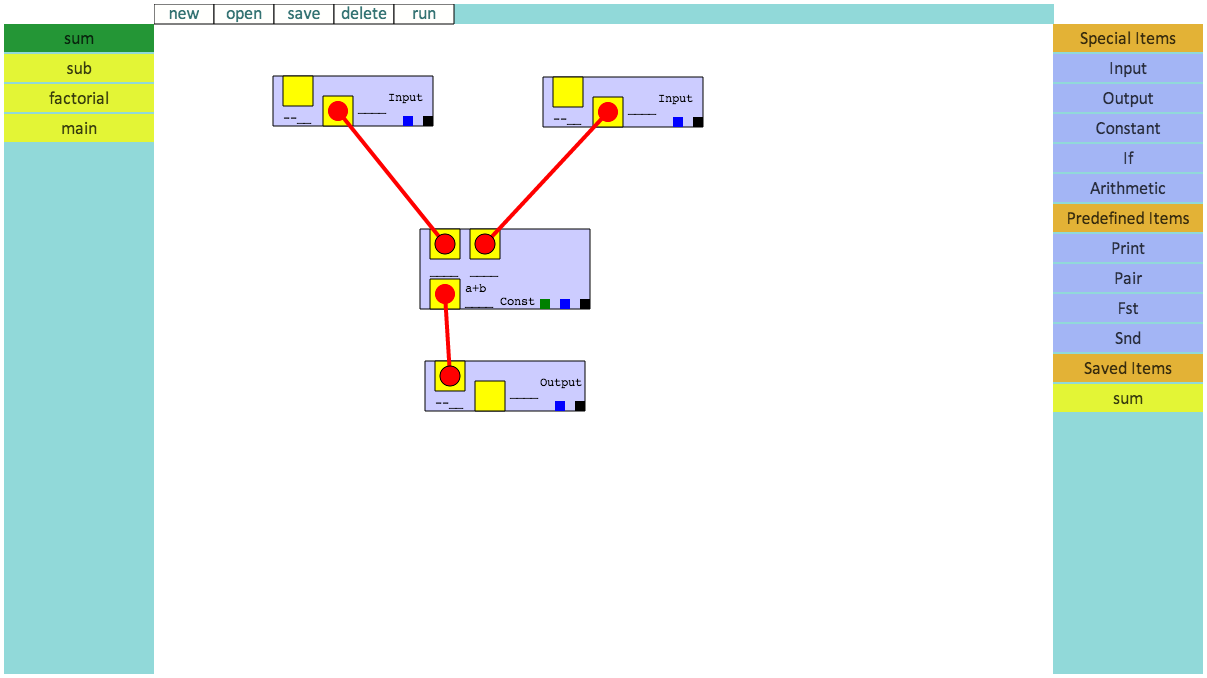
\includegraphics[width=.95\textwidth]{./images/gui.png} \\
\caption{The basic layout of the GUI.}\label{fig:gui}
\end{figure}
The top row of the GUI is the menu, which provides basic functionality
of manipulating user-defined definitions. Users are able to create new
function definitions, open existing function definitions, delete
unwanted definitions and save definitions as black-box functions. The
left side bar shows a list of user-defined functions, while on the
right side are the special definitions and predefined functions. If a
user-defined function is saved, it is also listed in the saved items
and is ready for to be used in other definitions. The central region
shows the function currently being constructed, which displays all the
member nodes of current definition. The member nodes are references to
either special definitions or functions (both predefined and
user-defined ones). Each node has input anchors and one output anchor,
except for nodes referring to special definitions such as input
definition or constant definition.

The central region only displays the function currently being defined,
and users can switch between different function definitions using the
left side bar. Items listed on the right side bar can be added to
current definition as member nodes. Nodes on current definition can
also be deleted if no longer needed.

The member nodes in a definition is connected by links between output
anchors and input anchors. A link represents using the output from the
one node as the input for the other node. A node can have output links
to multiple nodes, and a node having multiple inputs can link to
output anchors of different nodes.

Special nodes are added to represent special definitions. The node
representing \code{input} doesn't have any input anchor, while the
node for \code{output} can have only one input anchor. \code{constant}
node has a field for inputting the content of the constant, while
\code{recursion} node has the same number of inputs as current
definition. The \code{arithmetic} node is able to adjust its size and
number of inputs depending on the input expression.

\subsection{Error Reporting}

We identify the following errors and display them in a suitable manner:

\begin{itemize}
  \item Displayed as a alert box to the user:
  \begin{itemize}
    \item 'There must be one output.'
    \item 'There must be one input to main.'
  \end{itemize}
  \item Marks a node with a red outline and enables a tooltip, with an error message, to appear when the mouse hovers over the node:
  \begin{itemize}
    \item 'Incorrect number of inputs.'
    \item 'Input of main must be of type world.'
    \item 'Output of main must be of type world.'
  \end{itemize}
  \item Marks an edge in red and enables a tooltip, with an error message, to appear when the mouse hovers over the edge line:
  \begin{itemize}
    \item 'Input not connected.'
    \item 'Incompatible input types.' (The error message contains the two Types)
  \end{itemize}
\end{itemize}

For generic errors we have all three styles of error reporting. An example of each error style can be seen in figure~\ref{fig:errors}.

\begin{figure}[h!]
\center
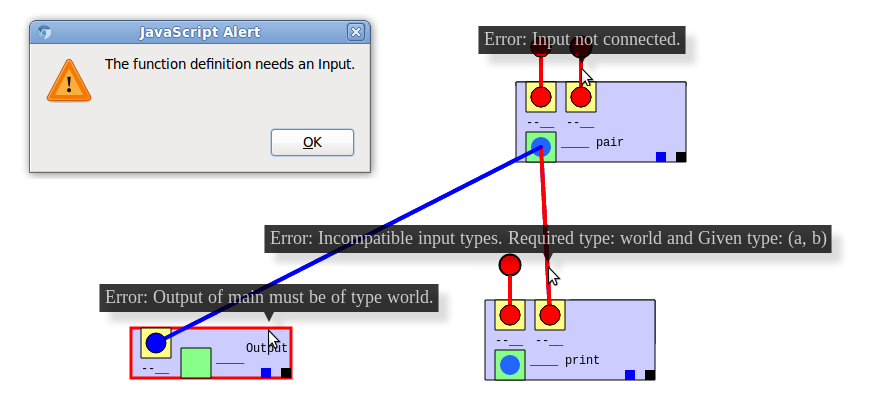
\includegraphics[width=0.95\textwidth]{./images/error_displays_cropped.png} \\
\caption{Several Error Messages.}\label{fig:errors}
\end{figure}

\section{Implementation Details}
\subsection{GUI}
The GUI is implemented in Javascript using the Kinetic Library\footnote{http://kineticjs.com/}. The implementation of the GUI has two major components: the basic GUI and the nodes. The basic GUI is the platform that support the definition-level operations, e.g. creation and deletion of function definitions and modification of the body of the definitions. The nodes are the basic elements that represent elementary functional units of a program, which are essentially references to existing definitions and appear as rectangular boxes in a definition body. 

The graphical elements in the GUI are organized in a hierarchical structure. The top level is a stage, which is the container for the layers representing each individual user-defined function. Each user defined function is associated with a layer, and all its member nodes reside in that layer. Definition level user interactions correspond to operations on the layers: switching between different definitions is equivalent to switching between layers, adding or removing functional units to a definition is represented by adding or removing nodes to a layer, and deleting a definition is accomplished by deleting a layer in the GUI.

The nodes used to represent single functional units are in the lowest level in the GUI hierarchy. They are represented by a group of graphical elements: input anchors, output anchor, bounding box and labels. Figure~\ref{fig:node} show a typical node structure. On the top are a set of input anchors, while the circle on the bottom of the bounding box is the output anchor. The labels are used for type information as well as showing the name of the referred definition. The blue square on the bottom-right corner is a short-cut for disconnecting all input/output links of the node, and the black one is used for deleting the node.
\begin{figure}[!ht]
\center
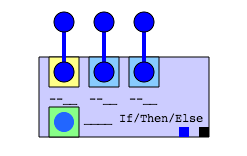
\includegraphics[width=0.3\textwidth]{./images/node} \\
\caption{A typical node.}\label{fig:node}
\end{figure}

Each node stores the definitions it is referring to as well as the definition it is in. The nodes also maintain a list of inputs and outputs by tracking the nodes they are connected to.

\clearpage

\subsection{Type-checking}
We represent each of the nodes as follows
\begin{center}
  \begin{tabular}{rrll}
    $u$ & ::= & $u\ \vec{i}\ o\ \vec{a}$ & --- program or functional unit
    \\
    $a$ & ::= & $o\ a$ & --- output node
    \\
    & $|$ & $i$ &  --- input node
    \\
    & $|$ & $f\ \vec{i}$ &  --- function node
    \\
    & $|$ & $c$ &  --- constant node
    \\
    & $|$ & $r\ \vec{i}$ &  --- recursion node
    \\
    & $|$ & $\code{if}\ a_1\ a_2\ a_3$ &  --- if node
    \\
  \end{tabular}
\end{center}
where $\vec{i}$ represents the list of input edges.

\begin{mathpar}
  \inferrule[Refl]{
    E(x) = \forall\alpha_1\dots\alpha_n.\tau
    \and
    Dom(\rho) \subseteq \{\alpha_1\dots\alpha_n\}
  }{
    E \vdash x : \rho(\tau)
  }
  \\
  \inferrule[Constant - Number]{}{E \vdash n : \type{number}}
  \and
  \inferrule[Constant - Boolean]{}{E \vdash b : \type{bool}}
  \and
  \inferrule[Constant - String]{}{E \vdash s : \type{string}}
  \\
  \inferrule[Input Node]{
    \alpha_x \text{ is fresh.}
  }{
    E \vdash i : \alpha_x
  }
  \and
  \inferrule[Output Node]{
    E \vdash a : \tau
  }{
    E \vdash o\ a : \tau
  }
  \and
  \inferrule[Instantiation]{
    E \not{\vdash} \alpha
    \and
    E \vdash a : \alpha
  }{
    E \vdash a : \tau
    \and
    E \vdash \alpha = \tau
  }
  \\
  \inferrule[Function Node]{
    E \vdash f : (\tau_1, \dots, \tau_n) \rightarrow \tau_r
    \and
    \forall n.\ E \vdash a_n : \tau_n
  }{
    E \vdash f\ (a_1, \dots, a_n) : \tau_r
  }
  \\
  \inferrule[If/Then/Else]{
    E \vdash a_1 : \type{bool}
    \and
    E \vdash a_2 : \tau
    \and
    E \vdash a_3 : \tau
  }{
    E \vdash \code{if}\ a_1\ a_2\ a_3 : \tau
  }
  \\
  \inferrule[Recursive Node]{
    E^{(\tau_1, \dots, \tau_n) \rightarrow \tau_r}
    \and
    \forall n.\ E \vdash i_n : \tau_n
  }{
    E \vdash r\ \vec{i} : \tau_r
  }
  \\
  \inferrule[Program]{
    \forall n.\ E^{(\tau_1, \dots, \tau_n) \rightarrow \tau_r} \vdash a_n : \bullet
    \and
    \forall n.\ E \vdash i_n : \tau_n
    \and
    E \vdash o : \tau_r
  }{
    E \vdash u\ (i_1, \dots, i_n)\ o_1\ (a_1, \dots, a_n)
    : Gen((\tau_1, \dots, \tau_n) \rightarrow \tau_r)
  }
  \\
  \inferrule[Program - Main]{
    \forall n.\ E^{\type{world} \rightarrow \type{world}} \vdash a_n : \bullet
    \and
    E \vdash i_1 : \type{world}
    \and
    E \vdash o : \type{world}
  }{
    E \vdash u\ (i_1)\ o_1\ (a_1, \dots, a_n)
    : \type{world} \rightarrow \type{world}
  }
\end{mathpar}
There are a few important points to note:
\begin{itemize}
\item Arithmetic nodes are treated identically as functional nodes.
\item Each node has exactly one type. Even if a type variable was
  created for it (such as with input nodes), that node can be
  instantiated to only one type and every other instance also uses
  that type.
\item Recursive nodes have exactly the type of the current translation
  unit. This means we do not support polymorphic recursion.
\item When a program is being used as the ``main'' program, it must
  satisfy the type rule {\sc Program - Main} instead of {\sc Program}.
\end{itemize}

The types of the builtin functions are listed in \ref{tab:pitemts}.
\begin{table}[h!]
\center
\begin{tabular}{c|c}
\hline
name & usage \\
\hline
\code{print} & $string \rightarrow world \rightarrow world$\\
\code{prompt} & $world \rightarrow (string, world)$\\
\code{pair} & $\forall \alpha,\beta.\ \alpha \rightarrow \beta \rightarrow (\alpha, \beta)$\\
\code{fst} & $\forall \alpha,\beta.\ (\alpha, \beta) \rightarrow \alpha$ \\
\code{snd} & $\forall \alpha,\beta.\ (\alpha, \beta) \rightarrow \beta$ \\
\code{stringofnumber} & $number \rightarrow string$\\
\code{stringofbool} & $bool \rightarrow string$\\
\code{single} & $\forall \alpha.\ \alpha \rightarrow List(\alpha)$ \\
\code{nil} & $\forall \alpha.\ List(\alpha)$ \\
\code{head} & $\forall \alpha.\ List(\alpha) \rightarrow \alpha$ \\
\code{tail} & $\forall \alpha.\ List(\alpha) \rightarrow List(\alpha)$ \\
\code{length} & $\forall \alpha.\ List(\alpha) \rightarrow number$ \\
\code{append} & $\forall \alpha.\ \alpha \rightarrow List(\alpha) \rightarrow List(\alpha)$ \\
\code{concat} & $\forall \alpha.\ List(\alpha) \rightarrow List(\alpha) \rightarrow List(\alpha)$
\end{tabular}
\caption{Predefined item types}\label{tab:pitemts}
\end{table}

\subsection{Evaluation}
Our evaluation strategy attempts to be pure, strict, and eager in all
cases where it makes sense. Nodes are evaluated only once, with
repeated evaluation available only through recursion. All arguments
are evaluated before the node itself is evaluated (with the important
exception of \code{if} expression). Furthermore, nodes which are not
required via this approach are {\em not} evaluated. This means
evaluation is most intuitively understood as a depth-first search for
a solution from the output node.

As mentioned above, \code{if} expressions do not respect the eager
evaluation of arguments. The conditional is evaluated first and then
only the branch selected is searched. This can be used with the
\type{world} type to implement flow control and with other types to
implement a base case for recursion.

\begin{mathpar}
  \inferrule[Function Node]{
    a_1 \rightarrow v_{n+1}
  }{
    f\ (v_1, \dots, v_n, a_1, \dots, a_n) \rightarrow f\ (v_1, \dots, v_{n+1}, a_2, \dots, a_n)
  }
  \\
  \inferrule[Function Application]{
    u \text{ is the program for } f
    \and
    \forall n.\ i_n \rightarrow v_n \implies u\ (i_1, \dots, i_n) \bullet \bullet \rightarrow v
  }{
    f\ (v_1, \dots, v_n) \rightarrow v
  }
  \\
  \inferrule[If - Cond]{
    a_1 \rightarrow v
  }{
    \code{if}\ a_1\ a_2\ a_3 \rightarrow \code{if}\ v\ a_2\ a_3
  }
  \and
  \inferrule[If - True]{
    a_2 \rightarrow v
  }{
    \code{if}\ \code{true}\ a_2\ \bullet \rightarrow v
  }
  \and
  \inferrule[If - False]{
    a_3 \rightarrow v
  }{
    \code{if}\ \code{false}\ \bullet\ a_3 \rightarrow v
  }
  \\
  \inferrule[Program]{
    o \rightarrow v
  }{
    u\ (i_1, \dots, i_n)\ o\ (a_1, \dots, a_n) \rightarrow v
  }
  \\
  \inferrule[Program - Main]{
    i \rightarrow \bullet \implies o \rightarrow v
  }{
    u\ i\ o\ (a_1, \dots, a_n) \rightarrow v
  }
\end{mathpar}

Recursion nodes and Arithmetic nodes are treated identically as
Function nodes, so their rules have been omitted to avoid
redundancy. Additionally, the exact evaluation of Arithmetic nodes has
been omitted because it follows simply from basic arithmetic.

Note that we have specified an evaluation order for arguments to
function nodes. This is not strictly needed; it is even undesirable if
the language was extended to include parallelism. It is included here
to specify in greater detail how our specific implementation performs;
arguments are evaluated left to right.

\subsubsection{Flaws}
The \type{world} type is used for sequencing, which works rather well
except for certain circumstances. Specifically, whenever data that
depends on a \type{world} value is used it introduces a dependency
that could cause undetermined execution order in a more liberal
implementation.

Because we use values and not thunks, this means even if the data is
only somewhat dependent we still trigger evaluation (such as
\type{world} being \code{pair}ed in a tuple). On the brighter side
however, these dependencies are quite visible at a glance due to the
graphical nature of the programs and can be avoided if they are deemed
problematic.

\subsection{Future Improvement}
One extension of the programming language that holds a lot of promise
is the idea of automatically wrapping sections of the program within a
special execution context (such as Haskell's Functors and
Monads). Take Haskell's \code{Maybe} monad for example.
\begin{center}
\begin{verbatim}
instance Monad Maybe where
  return x = Just x
  (>>=) m f = case m of Just x -> f x
                        Nothing -> Nothing
\end{verbatim}
\end{center}

This could easily translate to a dataflow language, automatically
lifting functions of type $a \rightarrow b$ to $\type{Maybe}\ a
\rightarrow \type{Maybe}\ b$ and automatically binding functions of
type $a \rightarrow \type{Maybe}\ b$. When multiple of these functions
are connected together, they could automatically form a context block
(like Haskell's \code{do}). This makes nondeterministic calculations
involving \code{List}s very clear: take the cartesian product of the inputs and accumulate all the results together.

As with all implicit features, there would need to be ways to control
this functionality. For example, what if you wanted to implement
\code{zip} instead of a general cross-product using \code{pair}? We
believe creating elegant controls for these features would be the most
difficult aspect of adding such a feature.

Unfortunately, due to project scope and time constraints we were
unable to further explore the design space. To truly take advantage of
such a feature, the user would need a fully-featured user-defined type
system which we did not implement in this project.

\end{document}
